\documentclass{article}
\usepackage{fullpage}
\usepackage{latexsym}
\usepackage{amssymb}
\usepackage{amsmath}
\usepackage[acronym]{glossaries}
%\usepackage{psfrag}
\usepackage[dvips]{graphicx}
\usepackage[latin1]{inputenc}
\usepackage{tikz}
\usetikzlibrary{shapes.geometric,arrows}


% Tikzstyle
\tikzstyle{startstop} = 
[
	rectangle, 
	rounded corners, 
	minimum width = 3cm, 
	minimum height = 1cm, 
	text centered, 
	draw=black, 
	fill=red!30
]

\tikzstyle{process} = 
	[
		rectangle, 
		minimum width=3cm, 
		minimum height=1cm, 
		text centered,
		draw=black, 
		fill=white!30
	]

\tikzstyle{arrow} = [thick,->,>=stealth]

\newacronym{AGCD}{AGCD}{Approximate Greatest Common Divisor}
\newacronym{APF}{APF}{Approximate Polynomial Factorisation}
\newacronym{CAGD}{CAGD}{Computer Aided Geometric Design}
\newacronym{GCD}{GCD}{Greatest Common Divisor}
\newacronym{SVD}{SVD}{Singular Value Decomposition}
\newacronym{SNTLN}{SNTLN}{Structured Non-Linear Total Least Norm}
\newacronym{CAD}{CAD}{Computer Aided Design}

%New commands
\newcommand{\GCD}{\textrm{GCD}}
\newcommand{\AGCD}{\textrm{AGCD}}
\newcommand{\ML}{\textrm{ML}}
\newcommand{\MDL}{\textrm{MDL}}
\newcommand{\rank}{\textrm{rank}}
\newcommand{\STLN}{\textrm{STLN}}
\newcommand{\SNTLN}{\textrm{SNTLN}}
\newcommand{\LSE}{\textrm{LSE}}
\newcommand{\SVD}{\textrm{SVD}}
\newcommand{\QR}{\textrm{QR}}
\newcommand{\APF}{\textrm{APF}}



\begin{document}
\begin{center}
Degree of an $\AGCD$ of two Bernstein polynomials
\end{center}
%
\date{}
%

\hrulefill

%\thispagestyle{empty}  % no page number is printed  on this page

\vspace{0.5cm}

This note describes the programs
%
\begin{center}
\texttt{o\_roots\_Univariate.m} 
and 
\texttt{o\_gcd\_Univariate\_2Polys.m}
\end{center}
%
\begin{enumerate}

	\item The first file is used in the computation of a polynomial's roots and corresponding multiplicities, where the given polynomial is in Bernstein form.
	
	\item The second file is used in the computation of the \gls{GCD} of two polynomials in Bernstein form.


\end{enumerate}


The programs are executed by typing
%
%
\begin{center}
\texttt
	{
	o\_roots\_Univariate
	(
		ex\_num, 
		emin, 
		emax, 
		mean\_method, 
		bool\_alpha\_theta, 
		low\_rank\_approx\_method, 
		apf\_method, 
		sylvester\_build\_method,
		rank\_revealing\_metric,
		deconvolution\_method\_hx,
		deconvolution\_method\_wx,
	)
	}

\texttt
	{
	o\_gcd\_2Polys\_Univariate
	(
		ex\_num, 
		emin, 
		emax, 
		mean\_method, 
		bool\_alpha\_theta, 
		low\_rank\_approx\_method, 
		apf\_method, 
		sylvester\_build\_method,
		rank\_revealing\_metric
	)}
\end{center}
%
 where
%
\begin{description}

	\item[ex\_num : ]
	(String) A string typically containing an integer, which defines the example to be run.
	
	\item[{emin} : ] (Float) Minimum signal : noise ratio
	
	\item[{emax} : ] (Float) Maximum signal : noise ratio
	
	\item[{mean\_method} : ] (String) Method used to compute the mean of the entries of the partitions of the Sylvester subresultant matrix
		\begin{description}
			\item[\texttt{None} : ] No mean method used
			\item[\texttt{Geometric Mean My Method} : ] Fast method 
			\item[\texttt{Geometric Mean Matlab Method} : ] Standard Matlab method
			\item[\texttt{Arithmetic Mean} : ] 
		\end{description} 

	
	\item[{bool\_alpha\_theta} : ] (Boolean)
		\begin{description}
			\item[\texttt{true} : ]  Preprocess polynomials
			\item[\texttt{false} : ]  Exclude preprocessing 
		\end{description}


	
	\item[{low\_rank\_approx\_method} : ] (String)
		\begin{description}
			\item[\texttt{None} : ] 
			\item[\texttt{Standard SNTLN} : ] 
			\item[\texttt{Standard STLN} : ]
			\item[\texttt{Root Specific SNTLN} : ] 
		\end{description}
	
	
	
	\item[{apf\_method} : ] (String)
		\begin{description}
			\item[\texttt{None} : ] 
			\item[\texttt{Standard Linear APF} : ]
			\item[\texttt{Standard NonLinear APF} : ]
		\end{description}


	\item[{Sylvester\_Build\_Method : }] (String)
		\begin{description}
			
			\item[{T} : ]
			The matrix 
			$
				T_{k}
				\left(
					f(x)
					,
					g(x)
				\right)
			$
			
			
			\item[{DT} : ]
			The matrix 
			$
				D^{-1}_{m+n-k}
				T_{k}
				\left(
					f(x)
					,
					g(x)
				\right)
			$
			
			\item[{DTQ} : ]
			The matrix
			$
				D^{-1}_{m+n-k}
				T_{k}
				\left(
					f(x)
					,
					g(x)
				\right)
				\hat{Q}
			$
			
			
			\item[{TQ} : ]
			The matrix
			$
				T_{k}
				\left(
					f(x)
					,
					g(x)
				\right)
				\hat{Q}
			$
			
			\item[{DTQ Rearranged} : ]
			The matrix 
			$
				S_{k}
				\left(
					f(x)
					,
					g(x)
				\right)
				=
				D^{-1}_{m+n-k}
				T_{k}
				\left(
					f(x)
					,
					g(x)
				\right)
				\hat{Q}
			$ where the entries are computed in a rearranged form.
			
			\item[{DTQ Denominator Removed} : ]
			$
				\tilde{S}
				\left(
					f(x)
					,
					g(x).
				\right)
			$
			
		\end{description}


	\item [rank\_revealing\_metric] (String)
		\begin{description}
			\item[Singular Values] : Compute the degree of the GCD using minimum singular values of the set of Sylvester subresultant matrices.
			
			\item[Max/Min Singular Values] : Compute the degree of the GCD using the ratio of maximum to minimum singular values of each Sylvester subresultant matrix.
			
			\item[R1 Row Norms] : Compute the degree of the GCD using the norm of the rows of the matrix R from the QR decomposition of each Sylvester subresultant matrix.
			
			\item[R1 Row Diagonals] : Compute the degree of the GCD using the diagonals of the matrix R obtained by the QR decomposition of each Sylvester subresultant matrix.
			
			\item[Residuals] : Compute the degree of the GCD using the minimum residual obtained by removing the optimal column of each of the Sylvester subresultant matrices.
		\end{description}
		
		
		
	\item [deconvolution\_method\_hx] (String)
		\begin{description}
		
			\item[Separate] :
			
			\item[Batch] :
			
			\item[Batch STLN] :
			
			\item[Batch Constrained] :
			
			\item[Batch Constrained STLN] :
			
		\end{description}
	
	\item [deconvolution\_method\_wx] (String)
		\begin{description}
			\item[Separate] :
			
			\item[Batch]  :
		\end{description}

%
\end{description}

\section{Examples}

Examples of executing the programs  are
%

\texttt
	{
		o\_gcd\_Univariate\_2Polys
		(
			`1',
			1e-10, 
			1e-12, 
			`Geometric Mean Matlab Method', 
			true, 
			`None', 
			`None', 
			`DTQ',
			`Minimum Singular Values'
		)}

\texttt
	{
		o\_roots\_Univariate
		(
			`1',
			 1e-12, 
			 1e-10, 
			 `Geometric Mean Matlab Method', 
			 true, 
			 `None', 
			 `None', 
			 `DTQ',
			 `Minimum Singular Values',
			 `Batch Constrained',
			 `Batch'
		)}

\section{Points of Interest}

\subsection{Other Variables}
Other less frequently changed variables are found in the file \texttt{SetGlobalVariables.m}

\begin{description}
	\item[SEED] (Int)Used in random number generation
	
	\item[PLOT\_GRAPHS] : (Boolean) 
		\begin{enumerate}
		\item true : Plot graphs
		\item false : Don't plot graphs
		\end{enumerate}
	
	\item[BOOL\_LOG] : (Boolean) Whether to use logs in the computation of the geometric mean
		\begin{enumerate}
		\item true
		\item false
		\end{enumerate}
	
	
	\item[GCD\_COEFFICIENT\_METHOD] (String)
		\begin{description}
			\item ux and vx
			\item ux
		\end{description}
	
	\item[MAX\_ERROR\_SNTLN] (Float)
	
	\item[MAX\_ITERATIONS\_SNTLN] (Int)
	
	\item[MAX\_ERROR\_APF] (Float)
		
	\item[MAX\_ITERATIONS\_APF] (Int)
		
	\item[GET\_HX\_METHOD] (String) Used in the computation of the set of polynomials $h_{i}(x)$ in the Tobey and Horowitz factorisation algorithm.
		\begin{description}
		\item[From Deconvolutions] : Deconvolve the set of polynomials $f_{i}(x)$
		\item[From ux] : The polynomials $h_{i}(x)$ are a by-product of the GCD computation. 
		\end{description}
	
	\item[DECONVOLVE\_METHOD\_HX\_FX] (String) 
	The deconvolution method used to obtain $h_{i}(x)$ from $f_{i}(x)$
		\begin{description}
			\item[Batch] 
			\item[Batch With STLN]
			\item[Batch Constrained]
			\item[Batch Constrained With STLN]
		\end{description}
	
	\item[DECONVOLVE\_METHOD\_WX\_HX] (String)
		\begin{description}
			\item[Separate]
			\item[Batch] 
		\end{description}
	
	\item[MAX\_ERROR\_DECONVOLUTIONS] (Float)
	
	\item[MAX\_ITERATIONS\_DECONVOLUTIONS] (Int)
	
	\item[PREPROC\_DECONVOLUTIONS] (Boolean)
	
\end{description}

\subsection{Limits}
The code makes frequent use of variables \texttt{t\_limits} and \texttt{k\_limits}. 
\begin{description}

	\item[\texttt{t\_limits} : ] In the computation of the factorisation of $\hat{f}_{0}(x)$, many \gls{GCD} computations are required to generate the sequence 
	$
		\hat{f}_{i}(x)
		=
		GCD
		\left(
			\hat{f}_{i-1}(x)
			,
			\hat{f}_{i-1}^{'}(x)
		\right)
	$. The degree of
	$
		GCD
		\left(
			\hat{f}_{i}(x)
			,
			\hat{f}_{i}^{'}(x)
		\right)
	$ is bound by the number of distinct roots of $\hat{f}_{i}(x)$, and the number of distinct roots is always less than or equal to the number of distinct roots of $\hat{f}_{i-1}(x)$. 
	
	\item[\texttt{k\_limits} : ] This variable defines the range of Sylvester subresultant matrices 
	$
		S_{k}
		\left(
			\hat{f}_{i}(x)
			,
			\hat{f}_{i}^{'}(x)
		\right)
	$ considered in the computation of the degree of the \gls{GCD}. By default this range is set between $1$ and $\min(m,n)$, however \texttt{limits\_t} can also be used since it is known that all subresultant matrices outside this range are known to be singular. 
\end{description}

\subsection{Computing the Degree of the GCD}
There are several methods considered for the computation of the degree of the \gls{GCD}. A global variable \texttt{SETTINGS.RANK\_REVEALING\_METRIC} defined in the file \texttt{SetGlobalVariables.m} determines which method is used.

\begin{description}
	
	\item[\texttt{Singular Values} : ] 
	
	\item[\texttt{R1 Row Norms} :]
	
	\item[\texttt{R1 Row Diagonals} : ]
	
	\item[\texttt{Residuals} : ]
	
\end{description}

%
\subsection{The Deconvolution Problem in the Polynomial Factorisation Algorithm}

The deconvolution functions can be tested away from the polynomial factorisation algorithm using the file \texttt{o\_Deconvolution.m}. The deconvolution methods considered are:
\begin{description}
	\item[\texttt{Separate} : ] 
	
	\item[\texttt{Batch} : ]
	
	\item[\texttt{Batch With STLN} : ]
	
	\item[\texttt{Batch Constrained} : ]
	
	\item[\texttt{Batch Constrained With STLN} : ]
\end{description}

\section{Code Flow}


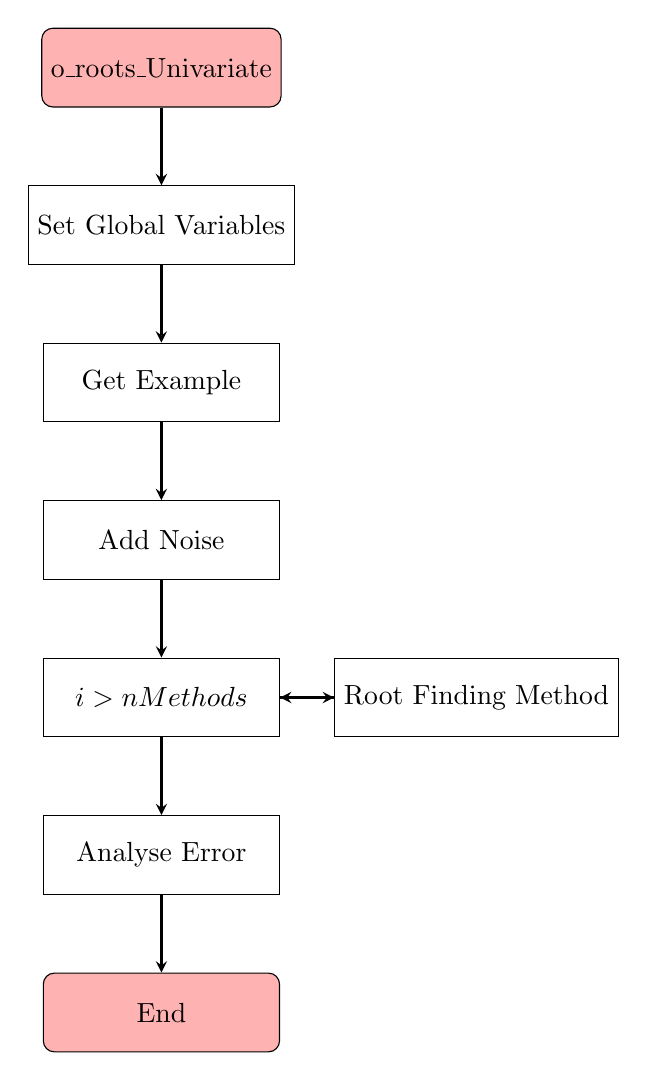
\begin{tikzpicture}[node distance=2cm]
	\node 
	(start) 
	[startstop] 
	{o\_roots\_Univariate};
	
	
	\node
	(SetGlobalVariables)
	[
		process,
		below of = start
	]
	{
		Set Global Variables
	}
	;
	
	\node
	(GetExample)
	[
		process,
		below of = SetGlobalVariables
	]
	{
		Get Example
	}
	;
	
	\node
	(AddNoise)
	[
		process,
		below of = GetExample
	]
	{
		Add Noise
	};	


	\node
	(Loop)
	[
		process,
		below of = AddNoise
	]
	{
		$i > nMethods$
	};


	\node
	(RootFindingMethod)
	[
		process,
		right of = Loop,
		xshift = 2cm
	]
	{
		Root Finding Method
	};
	
	\node
	(ErrorAnalysis)
	[
		process,
		below of = Loop
	]
	{
		Analyse Error
	};
	
	\node
	(End)
	[
		startstop,
		below of = ErrorAnalysis
	]
	{
		End
	};
	
	\draw [arrow] (start) -- (SetGlobalVariables);
	\draw [arrow] (SetGlobalVariables) -- (GetExample);
	\draw [arrow] (GetExample) -- (AddNoise);
	\draw [arrow] (AddNoise) -- (Loop);
	\draw [arrow] (Loop) -- (RootFindingMethod);
	\draw [arrow] (RootFindingMethod) -- (Loop);
	\draw [arrow] (Loop) -- (ErrorAnalysis);
	\draw [arrow] (ErrorAnalysis) -- (End);
	
\end{tikzpicture}



\end{document}





